% !TeX encoding = UTF-8
% !TeX program = pdflatex
% !BIB program = biber

%%% Um einen Artikel auf deutsch zu schreiben, genügt es die Klasse ohne
%%% Parameter zu laden.
\documentclass[]{lni}
%%% To write an article in English, please use the option ``english'' in order
%%% to get the correct hyphenation patterns and terms.
%%% \documentclass[english]{class}
%%

\usepackage[ngerman]{babel}
\usepackage{wrapfig}
\usepackage{csquotes}
\usepackage[
  backend=biber,
  style=LNI
]{biblatex}
\addbibresource{bib/Resiliency in System Architectures_File.bib}

% Titelformat Sections
\usepackage{titlesec}
\titlespacing{\section}{0pt}{\baselineskip}{0\baselineskip}
\titlespacing{\subsection}{0pt}{.5\baselineskip}{0\baselineskip}


\begin{document}
%%% Mehrere Autoren werden durch \and voneinander getrennt.
%%% Die Fußnote enthält die Adresse sowie eine E-Mail-Adresse.
%%% Das optionale Argument (sofern angegeben) wird für die Kopfzeile verwendet.
\title[Resilienz in Systemarchitekturen]{Resilienz in Systemarchitekturen}


%%%\subtitle{Untertitel / Subtitle} % if needed
\author[Robin Epple \and Timo Vollert]
{Robin Epple\footnote{DHBW Stuttgart Campus Horb, Studiengang Informatik, Florianstraße 15, 72160 Horb am Neckar,
Deutschland \email{i20010@hb.dhbw-stuttgart.de}} \and
Timo Vollert\footnote{DHBW Stuttgart Campus Horb, Studiengang Informatik, Florianstraße 15, 72160 Horb am Neckar,
Deutschland \email{i20033@hb.dhbw-stuttgart.de}}}


\startpage{1} % Beginn der Seitenzählung für diesen Beitrag / Start page
\editor{Herausgeber et al.} % Names of Editors
\booktitle{Advanced Software Engineering 2022} % Name of book title
\yearofpublication{2022}
%%%\lnidoi{18.18420/provided-by-editor-02} % if known
\maketitle


\begin{abstract}
% Was wollen Organisationen erreichen? - 24 Worte
Für Organisationen aller Art gehört es zu den obersten Prioritäten bestimmte interne und externe Prozesse am Laufen zu halten, um ihre Geschäftsziele zu erreichen. 
% Wieso spielt die Resilienz der Softwaresysteme dafür eine Rolle? - 19 Worte
Diese Prozesse werden im Zuge der Digitalisierung zunehmend abhängiger von Softwaresystemen. Infolgedessen muss moderne Software entsprechenden Resilienzanforderungen gerecht werden.
% Was ist die Schwierigkeit dabei? - 21 Worte
Die Schwierigkeit dabei ist, die Komplexität des Systems zu bewältigen, die aus der hohen Anzahl der Systemkomponenten und deren Vernetzungsgrad resultiert.
% Wie wird dem begegnet? - 32 Worte
In dieser Arbeit werden Prinzipien für verteilte Systeme behandelt, die es ermöglichen auch unter Ausfall von Teilsystemen die Funktionalität des Gesamtsystems zu erhalten.
Anschließend werden konkrete Entwurfsmuster vorgestellt, die diese Prinzipien implementieren.
% Summe 96 Worte
\end{abstract}

\begin{keywords}
Resilienz \and Resilience Management Model \and Normal Accident Theory \and Verteilte Systeme \and Entwurfsmuster
\end{keywords}


%%% Beginn des Artikeltexts
\section*{Einleitung} \label{intro}


Hin und wieder gehen Schlagzeilen durch die Medien, die von Ausfällen in der Infrastruktur oder in der Industrie berichten. Je nach Ausmaß und Schwere des Vorfalls können solche Ausfälle katastrophale Folgen für die Organisation selbst und alle Abhängigen bedeuten. Sowohl der Ausfall interner Strukturen, als auch von Produkten und Dienstleistungen stellt für viele Organisationen ein zu priorisierendes Risiko dar. Das Forschungsgebiet der Resilienz sucht Methoden, um Prozesse ausfallsicherer und verlässlicher zu machen. In Konsequenz der wachsenden Abhängigkeit von IT-Systemen übertragen sich diese Anforderungen auch auf die Software. Für die Entwicklung eines neuen Softwaresystems ist es heutzutage daher unabdingbar, entsprechende Resilienzanforderungen und -maßnahmen von Anfang an in den Entwurf einfließen zu lassen. 

Die Resilienz eines Systems zu gewährleisten ist ein komplexes und breites Themengebiet, das in enger Beziehung zu vielen anderen Fachbereichen steht: von der Unternehmensführung bis hin zum Systemhaus.

In diesem Beitrag soll daher zunächst die Bedeutung softwaretechnischer Maßnahmen für Resilienz in Organisationen erarbeitet werden. Im Anschluss wird sich die Arbeit darauf konzentrieren, wie ein Softwaresystem resilienter gemacht werden kann.

Im Zeitalter der Digitalisierung sind zwei Bewegungen in der Softwareentwicklung zu beobachten: Softwaresysteme werden umfangreicher und komplexer, gleichzeitig ist ein Ausfall zunehmend schlechter verkraftbar \cite[3]{CharlesPerrow.2000}. Das Forschungsgebiet, das sich mit dieser Problematik befasst heißt \glqq Resilience Engineering\grqq{} \cite{JonathanJohnson.20221101}. Bevor näher auf konkrete Maßnahmen in der Softwareentwicklung eingegangen wird, soll in den nächsten Abschnitten zunächst die Rolle der Softwareentwicklung in das breite Themenfeld der Resilienz eingeordnet werden.

\subsection*{Begriffsdefinition und Abgrenzung} \label{placement-definition}

Für diese Einordnung ist es wichtig, ein präzises Verständnis von dem Begriff Resilienz zu erhalten. Die Definitionen in der Literatur sind keineswegs einheitlich, vor allem aus dem Grund, dass sich das Themengebiet über viele verschiedene Fachbereiche erstreckt. Resilienz kann sich auf Software, Prozesse, Organisationen oder gar sozio-ökologische Systeme beziehen \cite[279]{Hickford.2018}. Über all diese Bereiche hinweg ist allerdings folgender Konsens erkennbar: \textit{Resilienz ist die Eigenschaft eines Systems, seine Funktionalität vor, während und nach einer Störung zu erhalten.} Was genau die Funktionalität des Systems ist, was unter \glqq Erhalt der Funktionalität\grqq{} verstanden wird und was eine Störung bedeutet variiert je nach Kontext \cite[279]{Hickford.2018}.

Für IT Systeme kann diese Definition konkretisiert werden, um sie von ähnlichen Eigenschaften abzugrenzen: \textit{Die Resilienz eines Softwaresystems beschreibt die Eigenschaft, seine Funktionalität unter partiellem Defekt in Toleranzgrenzen aufrecht zu erhalten und sie nach Überwindung des Defekts zu regenerieren} \cite[99]{Zhang.2010}. Resilienz lässt sich damit vor allem in einer Hinsicht von ähnlichen Eigenschaften wie Robustheit und Zuverlässigkeit abgrenzen: Die Resilienz eines Systems zeigt sich, wenn es partiell beschädigt ist \cite[99]{Zhang.2010}. 

Zuverlässigkeit beschreibt die Fähigkeit eines Systems, seine Funktionalität unbeschädigt und unter vorgesehenen Bedingungen zu liefern \cite[100]{Zhang.2010}. Die Robustheit eines Systems ist gefragt, wenn es zu unvorhergesehenen Störungen kommt, das System aber noch vollständig in Takt ist \cite[100]{Zhang.2010}. Erst wenn eine Störung die Zuverlässigkeit und Robustheit eines Systems übersteigt und es zum Ausfall einer oder mehrerer Komponenten kommt ist die Resilienz gefragt.

Im Zusammenhang mit diesen Definitionen ist es wichtig, sich Gedanken über den Betrachtungsrahmen zu machen: Ein System ist unbeschädigt, wenn alle seine Systemkomponenten die jeweilige Aufgabe erfüllen, die sie im System übernehmen sollen. Je nach Granularität der Betrachtung verschieben sich allerdings die Definitionen, was als \glqq Gesamtsystem\grqq{} und als \glqq Komponente\grqq{} betrachtet wird. Ist der Rahmen beispielsweise ein einzelner Server, so stellt der Ausfall einer Festplatte den Ausfall einer Komponente dar. In diesem Betrachtungskontext wäre ein RAID System als Resilienzmaßnahme zu betrachten, die den Erhalt der Systemfunktionalität unter partiellem Defekt gewährleistet. Wird als Rahmen allerdings ein Softwaresystem gewählt, das mehrere Geräte in einem Netzwerk umfasst, so ist der Server als ganzes eine Komponente. Das RAID System erhöht damit die Zuverlässigkeit dieser einzelnen Komponente, löst aber im Gesamtsystem kein Resilienzproblem. In diesem größeren Betrachtungskontext müssten Resilienzmaßnahmen den Ausfall des gesamten Servers kompensieren.

Diese Arbeit wird zur Einordnung mit einer gesamten Organisation als größtem Rahmen beginnen, um sich anschließend schrittweise in Softwarearchitekturen zu vertiefen. Vorab wird der nächste Abschnitt Grundlagen behandeln, die auf jeden Rahmen anwendbar sind.

\section*{Normal Accident Theory} \label{placement-NAT}

Bei näherer Betrachtung der Definitionen aus dem letzten Abschnitt liegt der Gedanke nahe, dass die Resilienz eines Systems überflüssig wird, wenn die Zuverlässigkeit und Robustheit der Komponenten nahe der Perfektion sind. 

Dieser Gedanke ist keineswegs neu und wird heute der High Reliability Theory (HRT) zugeordnet. In der HRT wird davon ausgegangen, dass mittels durchdachtem Management von Systemen und Prozessen Ausfälle von vorne herein ausgeschlossen werden können. Typische Maßnahmen in der Umsetzung der HRT sind eine hohe Priorisierung der Ausfallsicherheit in den Führungsebenen, dezentrale Autorität für schnelle Reaktionen, eine hohe Redundanz in Ressourcen und Personal und kontinuierliches Lernen an eigenen und fremden Fehlern mittels Personaltraining. \cite[100]{ThierryMeyer.2022}

Nachdem es im 20. Jahrhundert zunehmend zu Unfällen in scheinbar sicheren Systemen kam (beispielsweise im Kernkraftwerk von Three Mile Island) begann mit Charles Perrow eine Bewegung des Umdenkens \cite[9]{Perrow.2004}. Perrow begründete die Idee der \glqq Normal Accidents\grqq{}. Die Normal Accident Theory (NAT) hebt die Möglichkeit hervor, dass selbst bei scheinbar zur Perfektion gemanageten Systemen ein ungünstiges Zusammenspiel mehrerer Störungen zum Ausfall eines Teilsystemen führen können \cite[4]{CharlesPerrow.2000}. 

Hervorzuheben ist an dieser Stelle, dass die NAT keineswegs zu einer Vernachlässigung von Zuverlässigkeit und Robustheit aufruft. Fehler in einzelnen Komponenten werden von Perrow nicht als \glqq Normal Accidents\grqq{} klassifiziert. Die Vermeidung von Komponentenfehlern und damit ein zuverlässiges System sind vielmehr die Grundlage, auf der die NAT aufbaut \cite{Perrow.2004}. Die NAT weißt auf die Imperfektion des Menschen hin: Es darf niemals davon ausgegangen werden, dass ein System fehlerfrei ist, nur weil bisher keine Fehler entdeckt wurden. Es sollte immer die Möglichkeit in Betracht gezogen werden, dass Umstände auftreten, die vorher nicht berücksichtigt wurden, und dass es bei ungünstigen Kombinationen zum Ausfall von (Teil-)Systemen kommen kann.

Die NAT verlangt also, aufbauend auf einem zuverlässigen System den Fehlerfall zu erwarten. Sollte eine Komponente ausfallen, muss das System reagieren, um diesen Ausfall zu kompensieren. Ein Komponentenfehler soll nicht zu kaskadieren Abhängigkeitsfehlern führen.

Die Maßnahmen zur Resilienzsteigerung lassen sich aus den Ursachen der \glqq Normal Accidents\grqq{} ableiten. Die Arbeiten von Perrow führen diese Fehler auf zwei Dimensionen zurück: Die Komplexität der Interaktionen in einem System und die Enge der Kopplung zwischen Systemkomponenten \cite{Perrow.2004}.

Die Komplexität eines Systems wird definiert durch die Anzahl, Anordnung und Ersichtlichkeit der Interaktionen zwischen seinen Komponenten. Sie spielt vor allem aufgrund der menschlichen Imperfektion eine Rolle in der NAT. Je linearer die Interaktionen zwischen den Komponenten sind, desto übersichtlicher wird das System für menschliche Betrachter \cite[72]{CharlesPerrow.2000}. In einem linearen Fluss ist es einfach, die Auswirkungen von lokalen Problemen auf benachbarte Komponenten zu überblicken und Gegenmaßnahmen einzuplanen. Je komplexer und undurchsichtiger das Netzwerk aus Interaktionen ist, desto wahrscheinlicher wird es, dass bestimmte Umstände und Aspekte übersehen werden, die Katastrophenpotential bergen.

Die Eigenschaft der Kopplung beschreibt, wie starr die Abhängigkeiten zwischen den Komponenten sind. Je enger die Kopplung desto weniger Handlungsspielraum hat eine Komponente. Fällt ein Interaktionspartner aus, dann führt eine starre Abhängigkeit unausweichlich zu Folgefehlern. Es kommt zu sich ausbreitenden Abhängigkeitsfehlern, die nur mit einer zentralen Maßnahme gestoppt und behoben werden können. Lose Kopplungen hingegen erlauben es einem System, lokal alternative Prozessabläufe einzuleiten um die verlorene Abhängigkeit zu kompensieren. Man spricht von einer dezentralen Fehlerbehandlung. \cite[101]{ThierryMeyer.2022}



\begin{figure}[ht]
    \centering
    \hspace{1.7cm}
    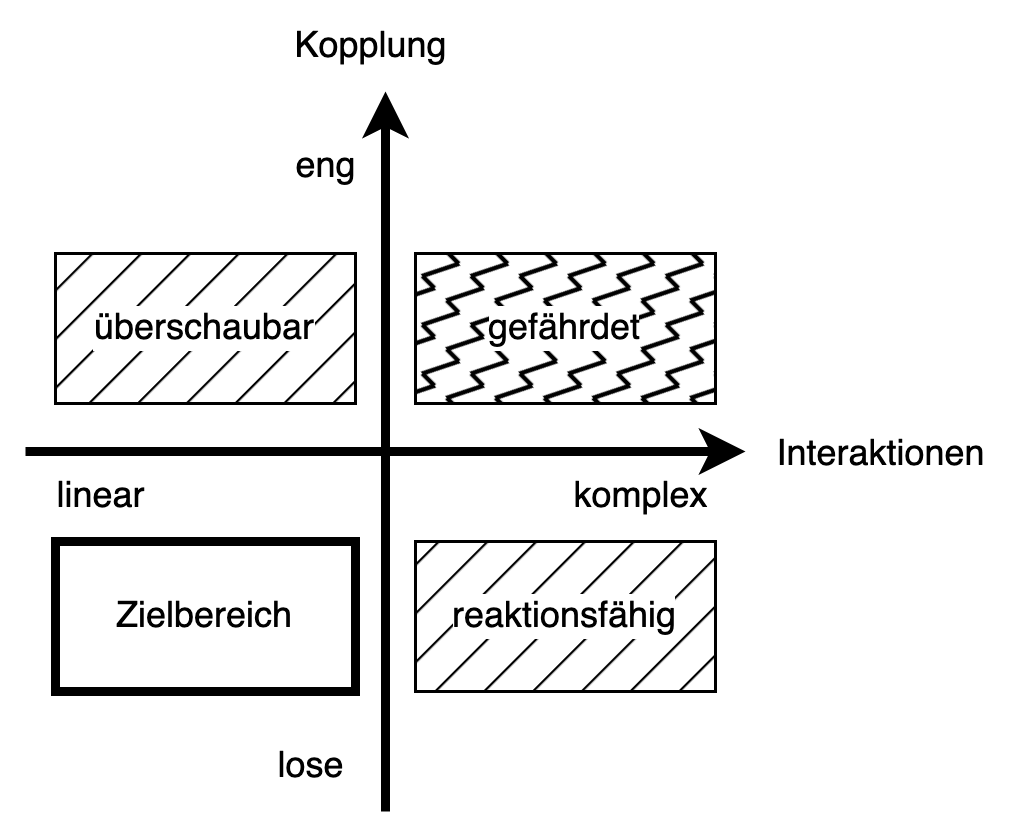
\includegraphics[width=.6\textwidth]{images/NatDimensions.drawio.png}
    \caption{Interaktionsdimensionen NAT}
    \label{fig:NatDimensions}
\end{figure}



Bildet man aus diesen beiden Eigenschaften ein Koordinatensystem, dann lassen sich die Systeme in vier Quadranten einteilen (siehe Abbildung \ref{fig:NatDimensions}) \cite[97]{CharlesPerrow.2000}. Ein resilientes System strebt möglichst lineare, übersichtliche Interaktionen bei gleichzeitig loser Kopplung an \cite[101]{ThierryMeyer.2022}. Lässt sich eine enge Kopplung nicht vermeiden, sollte diese durch möglichst einfache Interaktionen ausgeglichen werden und umgekehrt. Wird das System in den Quadranten für enge Kopplung und komplexe Interaktionen eingeordnet, ist das ein Warnsignal.

Im Kontext der resilienten Softwareentwicklung können zwei Lehren aus der NAT gezogen werden: Um Abhängigkeitsfehler beim Ausfall einer Komponente zu vermeiden benötigen die Prozessabläufe Ausweichmöglichkeiten und lokalen Spielraum. Lose Kopplungen erfordern redundante Funktionalität im System.

Die zweite Lehre betrifft die Komplexität der Interaktionen. Natürlich kann innerhalb des Softwaresystems auf möglichst übersichtliche Prozessabläufe geachtet werden. Entscheidend ist aber, dass Softwaresysteme letztendlich nur ein Teil von größeren Systemen sind. Um die Komplexität nachhaltig zu reduzieren, müssen ganze Geschäftsprozesse überarbeitet werden, nicht nur die Software.


\section*{Resilience Management Model} \label{placement-RMM}


Dieser Gedanke führt unweigerlich zum Resilienzmanagement. Resilienzmanagement ist dafür verantwortlich, die Kerngeschäfte einer Organisation abzusichern und zentrale Unternehmenstätigkeiten unter allen Umständen am Laufen zu halten. Es betrifft also alle Komponenten des Systems innerhalb einer Organisation. Dieses Kapitel soll einen Überblick über das breite Themengebiet geben, um anschließend einzuordnen welche Rolle Software in einem resilienten Prozess übernehmen muss, und welche Anforderungen an das System daraus resultieren.

Das Resilience Management Model (RMM) von CERT will einen Leitfaden für Unternehmen bieten, mit dem priorisierte Leistungen aufrecht erhalten werden können. Die Informationen im nachfolgenden Abschnitt referenzieren die Originalpublikation \cite{CERT_RMM} sofern nicht anders angegeben. Sinngemäß übersetzt lautet die Definition für Resilienzmanagement in dem Standard wiefolgt:

\begin{quote}
    Resilienzmanagement umfasst Prozesse und Praktiken einer Organisation, die Strategien entwerfen, entwickeln, implementieren und steuern, die dem Schutz und Erhalt von Dienstleistungen, Wirtschaftsgütern oder anderen Prozessen mit hohem Wert dienen.
    \cite[19]{CERT_RMM}
\end{quote}

Die Definition macht bereits deutlich, dass das Management einen anderen Blickwinkel auf das Thema Resilienz hat. Ressourcen sind nur ein Teil der Zielmenge von Schutzmaßnahmen. Vorrangig ist zunächst, schützenswerte Wirtschaftsgüter zu identifizieren und notwendige Maßnahmen einzuleiten. Abbildung \ref{fig:RmmServicesToAssets} veranschaulicht, wie ein Unternehmen zu Strategien und Maßnahmen finden kann, die die Unternehmensresilienz steigern.



\begin{figure}[ht]
    \centering
    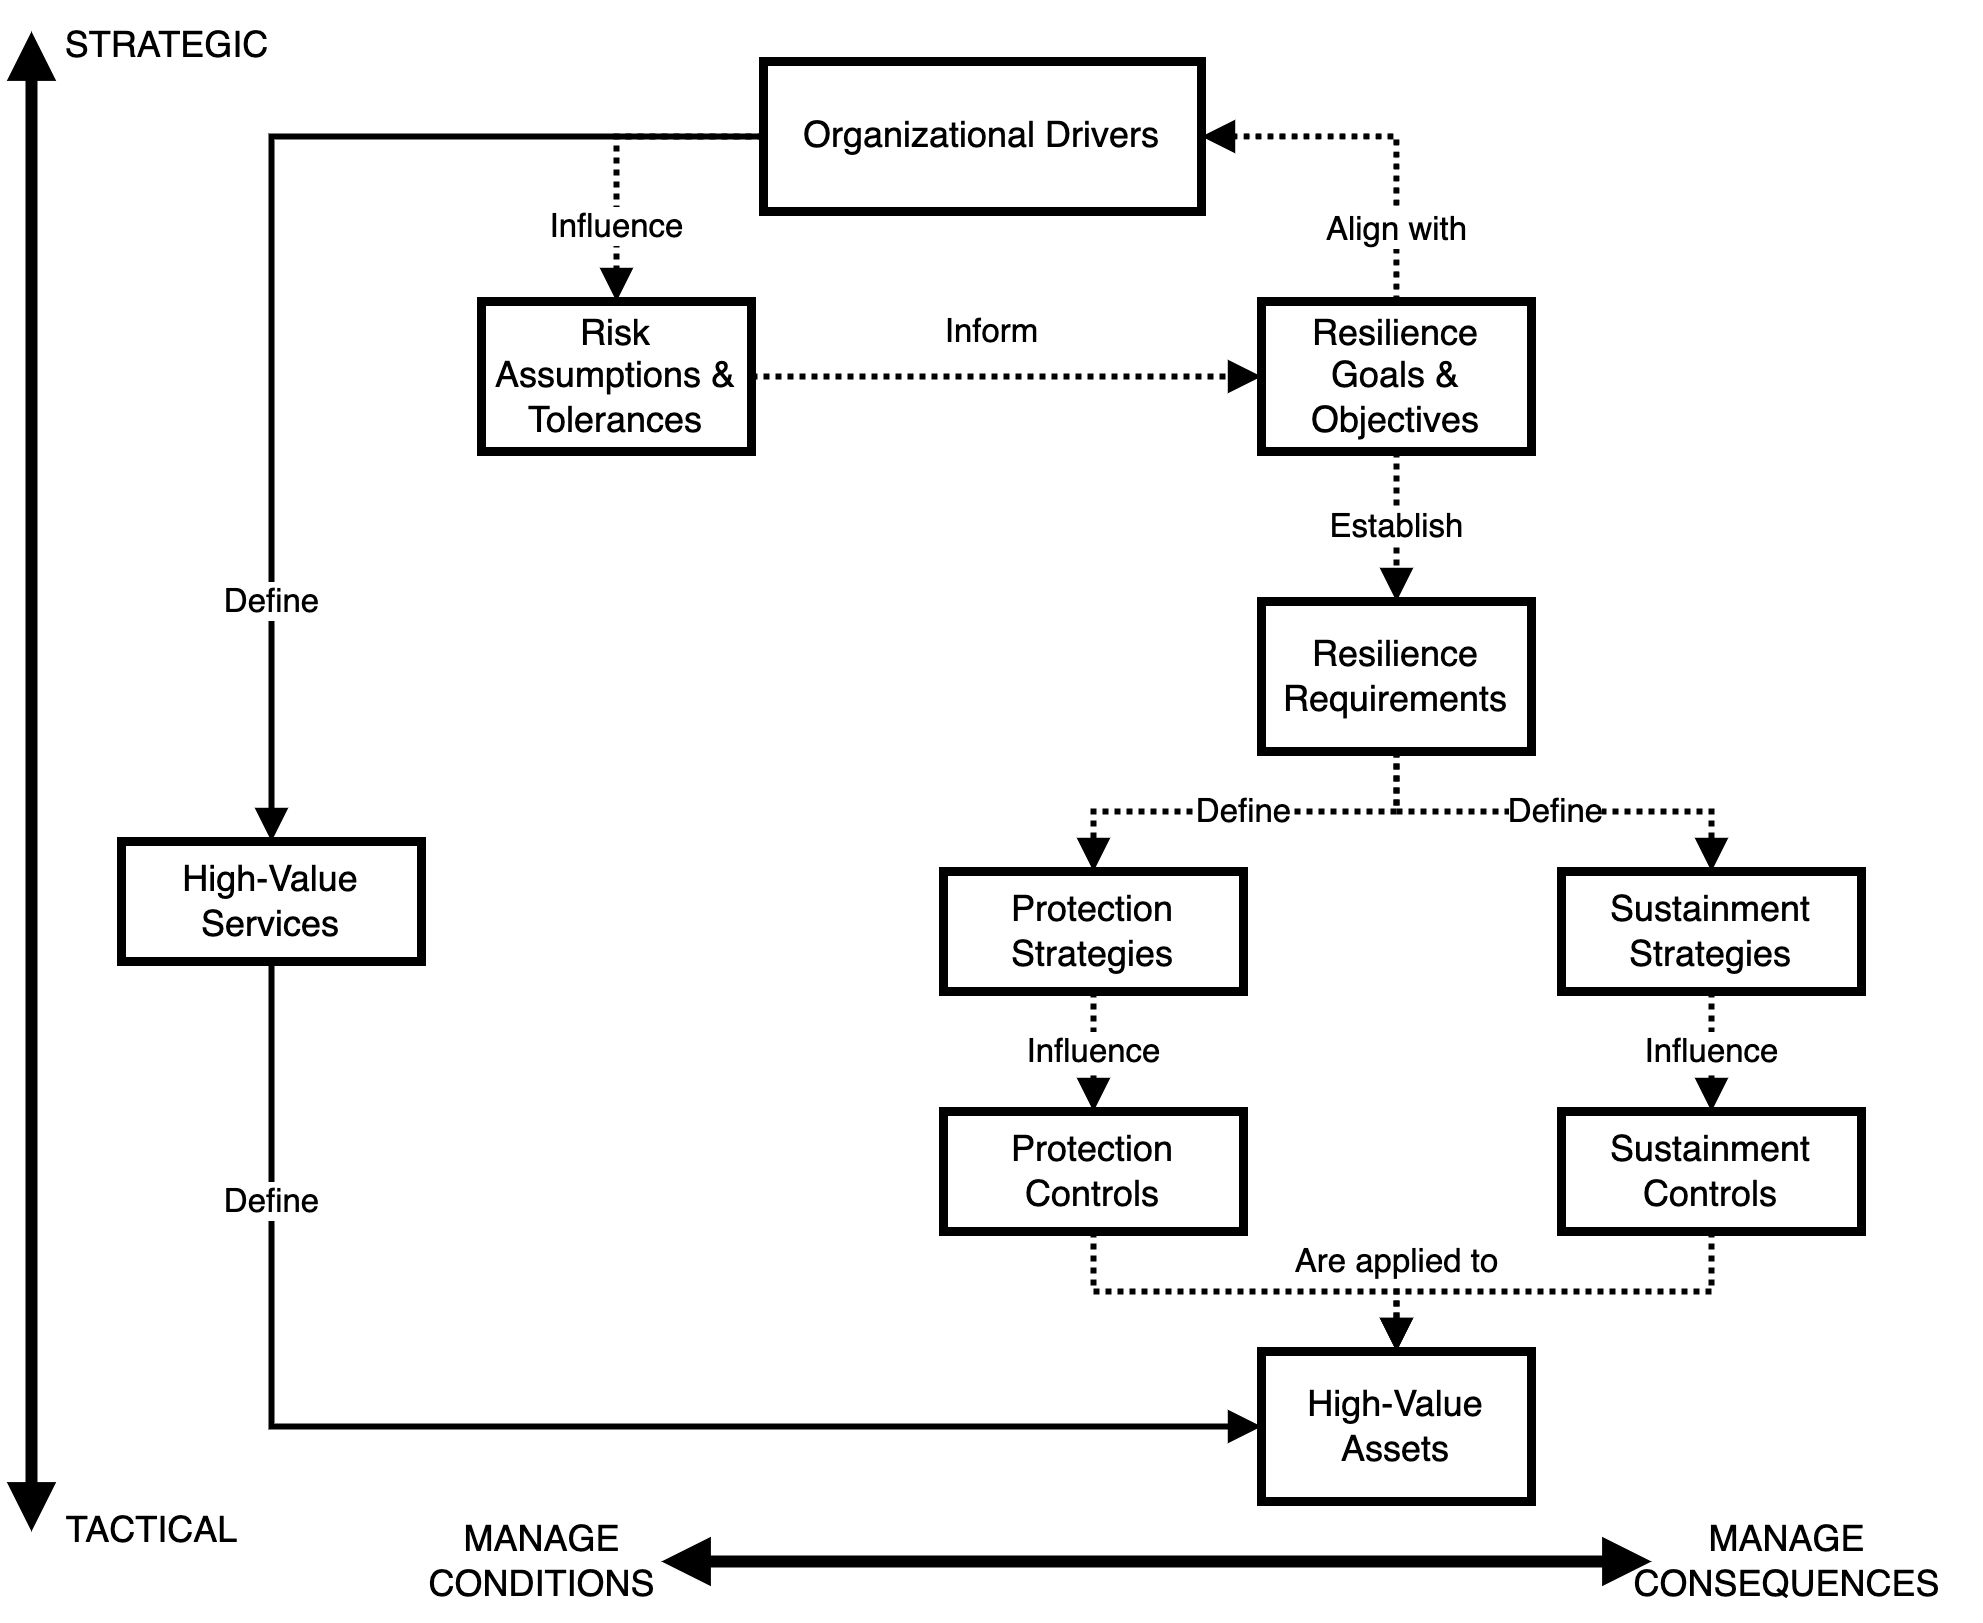
\includegraphics[width=.9\textwidth]{images/RMM_strategy_deriviation_graph.drawio.png}
    \caption{Ableiten von Resilienzmaßnahmen aus Unternehmenszielen. Nachbildung von \cite[S. 26, Figure 9]{CERT_RMM}.}
    \label{fig:RmmServicesToAssets}
\end{figure}



An oberster Stufe der Grafik stehen Organisationstreiber. Das sind Strukturen, die ein förderndes Umfeld für die Organisation entwickeln oder erhalten wollen \cite{NationalImplementationResearchNetwork.}.

Davon ausgehend verfolgt der linke Pfad in der Grafik den Prozess, einzelne schützenswerte Ressourcen aus übergeordneten Unternehmenszielen abzuleiten. In diesem Prozess definiert das RMM drei Ebenen: Dienstleistungen, Prozesse und Ressourcen. 

Dienstleistungen sind das eigentliche Objekt, das es zu schützen gilt. Darunter kann jede Tätigkeit einer Organisation verstanden werden: Von internen Managementstrukturen über Produktionstätigkeiten bis hin zu externen Dienstleistungen bei Kunden. Es gilt die Bedeutung der Dienstleistung für den Erhalt der Tätigkeit des Unternehmens zu bewerten. Mit diesen Informationen kann eine Priorisierung der Leistungen vorgenommen werden.

Eine Dienstleistung besteht aus einem oder mehreren Prozessen. Prozesse sind beliebige Geschäftsprozesse. Sie bestehen aus Aktivitäten, die manuelle Aufgaben, vollautomatisierte Prozessschritte oder interne und externe Kommunikation abbilden können.

Prozesse sind der Hauptfokus von RMM, da sie konkrete Arbeitsabläufe darstellen, die analysiert und überarbeitet werden können. In der Übersichtsgrafik \ref{fig:RmmServicesToAssets} sind sie allerdings nicht abgebildet, da Prozesse letztlich \glqq nur\grqq{} konkrete Umsetzungen der Dienstleistungen sind. Resilienzmaßnahmen schützen Prozesse, um Dienstleistungen zu erhalten.

Im Ableitungsprozess stellen Prozesse dennoch einen wichtigen Schritt dar, da sie Dienstleistungen mit ihren Abhängigkeiten verbinden. Abhängigkeiten sind beliebige Ressourcen der Organisation. Über die Prozesse können Ressourcen identifiziert werden, die für den Erhalt der Unternehmenstätigkeit besondere Bedeutung besitzen.

Ressourcen werden im Standard in vier übergeordnete Kategorien eingeteilt:

\begin{enumerate}
    \item Personen, die beteiligt oder verantwortlich sind.
    \item Informationen, die der Prozess benötigt oder generiert.
    \item Technologien, die für die Durchführung benötigt werden.
    \item Einrichtungen oder Gebäude, von denen der Prozess abhängt.
\end{enumerate}

Softwaresysteme sind der Kategorie \glqq Technologien\grqq{} zuzuordnen. Abbildung \ref{fig:ServicesToResources} bildet den Zusammenhang von Dienstleistungen und Ressourcen ab. Wichtige Ressourcen können auch Teil mehrerer priorisierter Dienstleistungen oder Prozesse sein.



\begin{figure}[ht]
    \centering
    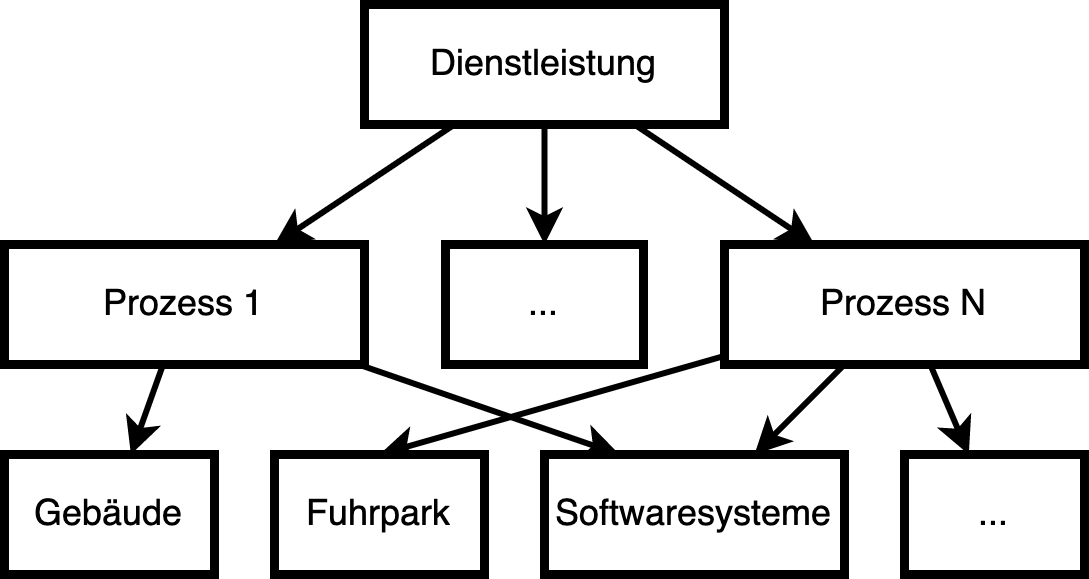
\includegraphics[width=.5\textwidth]{images/ServicesToResources.drawio.png}
    \caption{Schützenswerte Ressourcen von priorisierten Dienstleistungen ableiten.}
    \label{fig:ServicesToResources}
\end{figure}



In Abbildung \ref{fig:RmmServicesToAssets} führt noch ein zweiter Pfad von den Organisationstreibern zu den priorisierten Ressourcen. Er spiegelt den Prozess wieder, konkrete Schutzmaßnahmen zu entwickeln.

In diesem zweiten Pfad wird deutlich, dass Resilienzmanagement alle Ebenen eines Unternehmens betrifft. Er hat seinen Ursprung in der strategischen Ebene der Unternehmensführung und zieht sich in der Grafik bis in die taktische Ebene. Die Umsetzung ist in dieser Grafik nicht abgebildet, ist aber ebenso Teil der Kette.

Auf strategischer Ebene findet sich auf der linken Seite der Punkt \glqq Risikoannahmen und Toleranzen\grqq{}, der die Informationsgrundlage für \glqq Resilienzziele\grqq{} bildet. Hier wird der Enge Zusammenhang von Resilienzmanagement und Risikomanagement ersichtlich. Resilienzmanagement ist eine Methode, um identifizierten Risiken zu begegnen. 

Sind die Resilienzanforderungen einmal definiert, teilt das RMM den Pfad in die Entwicklung schützender und erhaltender Strategien. 

Schützende Strategien sollen erreichen, dass Ressourcen von Grund auf weniger Störungen ausgesetzt sind. Für Resilienz rund um Softwaresysteme bedeutet das, dass die Software nicht alle Störungen selbst abfangen muss. Es kann auch Mechanismen in der Betriebsumgebung geben, die viele Gefahren abblocken, bevor sie das System erreichen.

Erhaltende Strategien sollen die Funktionalität der Ressource in Toleranzgrenzen aufrechterhalten, während sie einer Störung ausgesetzt ist. Diese Definition macht zum einen deutlich, dass auch im Störungsfall nicht zwingend die Ressource, also das Softwaresystem selbstständig reagieren können muss. Wie in Abschnitt \glqq Theoretische Prinzipien\grqq{} ersichtlich werden wird, sind einige Resilienzanforderungen an ein Softwaresystem sehr komplex. Es kann eine valide Entscheidung sein, die Komplexität der Software zu reduzieren, indem andere begleitende Systeme die entsprechenden Eigenschaften sicherstellen.

Zu den Strategien werden auf taktischer Ebene konkrete Maßnahmen definiert, die auf die Ressourcen angewendet werden. Insgesamt macht dieser Pfad deutlich, dass beim Resilienzmanagement Softwaresysteme nicht isoliert betrachtet, sondern in ihren Kontext der Geschäftsprozesse eingeordnet und als Gesamtsystem resilienter gemacht werden. Neben der Software spielen Personal, Management, Umgebungsbedingungen und viele weitere Faktoren eine Rolle. Im Folgenden wird sich diese Arbeit allerdings konkret Software und dessen Entwicklungsprozess konzentrieren.

\subsection*{Softwareentwicklung} \label{placement-software}

Der Standard RMM identifiziert insgesamt sechsundzwanzig Prozessräume in vier Kategorien. Resilienz in Software und Softwaresystemen wird einem davon zugeordnet: \glqq Resilient Technical Solution Engineering\grqq{} in der Kategorie \glqq Engineering\grqq{} \cite[31]{CERT_RMM}.

RMM selbst gibt wenig konkrete Maßnahmen vor, die ein Unternehmen umsetzen kann oder muss. Stattdessen gibt es Anreize, was die Führungsebene beim Resilienzmanagement beachten muss. 

Ein hohes Gewicht bekommt die Ermahnung, dass effektive Resilienzmaßnahmen bereits von Beginn an in den Entwicklungsprozess neuer Software einfließen müssen \cite[178]{CERT_RMM}. Um Resilienz effektiv im Unternehmen zu etablieren wird empfohlen, nicht jedes System einzeln zu behandeln, sondern Richtlinien für die Softwareentwicklung zu definieren, die bei jedem Projekt eingehalten werden \cite[179]{CERT_RMM}.

RMM definiert nur vage, was in diesen Richtlinien enthalten sein sollte, es wird aber auf verschiedene Quellen mit guter Reputation verwiesen, die als Orientierung dienen können. Eine davon ist der Microsoft Security Development Lifecycle (SDL), der nachfolgend näher beleuchtet werden soll \cite[180]{CERT_RMM}.  

Dieser Standard macht deutlich, dass Resilienzmanagement ebenfalls eng mit Sicherheitsmanagement zusammen hängt.

SDL definiert zwölf Praktiken, die bei der Softwareentwicklung beachtet werden sollten \cite{MSDL}. Nachfolgend werden diese Praktiken in vier Faktoren klassifiziert: beteiligte Personen, Anforderungen, Umfeld und Tests.

\paragraph{Practice \#1: beteiligte Personen}
Die Basis für wirksame Resilienzmaßnahmen ist, dass sie von betroffenen Mitarbeitern umgesetzt werden. Der erste Faktor ist daher Personaltraining in allen beteiligten Bereichen, von der Entwicklung bis hin zum Produktmanagement. Gleichzeitig steigert das Training das Bewusstsein für Gefahren und die Notwendigkeit von Absicherungen.

\paragraph{Practice \#2-6: Anforderungen}
Der zweite Faktor ist die Analyse der Anforderungen an das System. Es müssen Gefahren ermittelt, eventuell modelliert und anschließend in Anforderungen umgesetzt werden. Um die Erfüllung der Anforderungen sicherzustellen ist es sinnvoll, Metriken zu definieren, die bestanden werden müssen. Für die konkrete Umsetzung ist es häufig sinnvoll, globale Designentscheidungen und Implementierungspraktiken zu definieren, beispielsweise die Entscheidung für bestimmte Sicherheitsstandards.

\paragraph{Practice \#7-8: Umfeld}
Die dritte Kategorie von Praktiken ruft dazu auf, verwendete Werkzeuge und Drittherstellerkomponenten unter die Lupe zu nehmen, um festzustellen, ob sie den Ansprüchen genügen. Gleichzeitig sollte ein Inventar über verwendete Drittherstellersoftware gehalten und Maßnahmen definiert werden, um einschreiten zu können falls ein Sicherheitsproblem bekannt wird.

\paragraph{Practice \#9-12: Tests}
Der letzte Faktor ist die Sicherstellung, dass die Software den Anforderungen entspricht. Hier können verschiedene Testmethoden zum Einsatz kommen, beispielsweise statische und dynamische Sicherheitstests und Penetrationstests. Zusätzlich ist es eine wertvolle Maßnahme, einen Standardprozess für die Reaktion auf Probleme im Einsatz zu definieren.



\section*{Angestrebte Eigenschaften} \label{design-properties}

Um resilient zu sein muss ein Softwaresystem gewisse Eigenschaften erfüllen.
Diese definiert \cite{ThierryMeyer.2022} als die Eigenschaften Kapazität, Flexibilität, Toleranz und Kohäsion.

\paragraph{Kapazität}
Die Kapazität eines Softwaresystems beschreibt die Fähigkeit Bedrohungen zu widerstehen.
Um das zu erreichen soll das System gewisse Belastungen absorbieren können.
Dazu gehört auch, dass sowohl physische, als auch funktionale Redundanzen existieren, auf welche ausgewichen werden kann.
%Single Point of Failure
Im Rahmen der Resilienz kann die Kapazität eines Systems überschritten werden.
In dem Fall verlässt sich das System darauf, dass sich das System anhand der drei weiteren Eigenschaften wieder erholt.

\paragraph{Flexibilität}
In Angesicht einer Bedrohung ermöglicht die Flexibilität dem System sich zu restrukturieren.
So kann dieses bei Bedarf die eigene Architektur anpassen um beispielsweise funktionale Redundanzen zu verwenden.
Für diese kann es nötig sein, dass der Programmablauf angepasst werden muss.
Dafür ist es sehr hilfreich, wenn das System eine lose Kopplung realisiert.
So können die einzelnen Komponenten mit weniger Aufwand restrukturiert werden.

\paragraph{Toleranz}
Wird die Kapazität eines Systems überschritten, so gewährt die Toleranz eine geordnete Reduktion der Funktionen.
Wie bereits bei der Flexibilität hilft hier ein lose gekoppeltes System.
Dieses ermöglicht die ausgefallenen Komponenten einfacher aus dem Programmablauf herauszunehmen, so dass sich die Ausfälle auf einen Systemteilausfall beschränken.
Das System soll zudem in der Lage sein sich von der Reduktion zu erholen, indem die Funktionen wiederhergestellt oder ersetzt werden.

\paragraph{Kohäsion}
Durch die Kohäsion eines Systems wird der totale Systemzerfall unterbunden.
Das System bleibt vor, während und nach einer Bedrohung funktionstüchtig.
Dafür muss eine Basiskommunikation der Systemknoten aufrecht erhalten werden.
So kann ermöglicht werden, dass sich das System eigenständig erholt.


\section*{Theoretische Prinzipien} \label{design-prinicpals}

In \cite[104]{Zhang.2010} werden fünf theoretische Prinzipien aufgelistet, nach welchen ein resilientes System modelliert werden sollte, welches diese Eigenschaften besitzt.
Diese Prinzipien dienen als Richtlinien für ein theoretisch ideal resilientes System.
Eine vollständige Umsetzung dieser Prinzipien ist in vielen Systemen unrealistisch durch eine reine Softwarelösung zu realisieren.

Darum werden in der Realität viele der Funktionen durch menschliche Aktoren ausgeführt.
Aber auch mit menschlichen Aktoren dienen sie als Richtlinien, welche Elemente ein System besitzen muss, um resilient zu sein.

Die Prinzipien beschreiben ein Zusammenspiel von Hard- und Software in einem System, welches modular und anpassbar ist.
In Abbild \ref{fig:ResilienzPrinzipien} wird das Zusammenspiel dieser Prinzipien abgebildet.

\begin{figure}
    \centering
    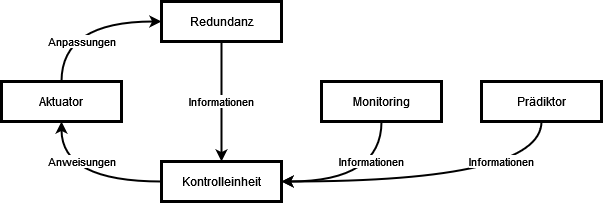
\includegraphics[width=.9\textwidth]{images/Resilienz Prinzipien.drawio.png}
    \caption{Zusammenspiel der fünf Prinzipien. Adaption von \cite[Figure 5, S. 109]{Zhang.2010}.}
    \label{fig:ResilienzPrinzipien}
\end{figure}

\paragraph{Redundanz}
Ein resilientes System sollte mit einem bestimmten Grad an Redundanz entworfen werden.
Dabei sollten physische und funktionale Redundanz implementiert werden.
Diese erhöhen die Kapazität des Systems.

Die Redundanz eines Systems misst sich darin, dass Systemfunktionen jeweils von mehreren Komponenten ausgeführt werden können.
Diese unterteilt sich in die funktionale und die physische Redundanz.
Die funktionale Redundanz bedeutet, dass einzelne Funktionen mehrfach umplementiert werden.
Dabei können die Implementierungen voneinander abweichen, lediglich die zu erfüllende Funktion muss die gleiche sein.
Bei der physischen Redundanz geht es darum, dass das System auf mehrere Maschinen verteilt ist.
So kann das System auch bei dem Ausfall der Hardware die Funktion aufrecht erhalten.

\paragraph{Monitoring}
Ein resilientes System sollte ein Monitoring besitzen, welches verantwortlich ist für die zeitliche und räumliche Überwachung der Systemfunktionen und Arbeitsleistung, Überwachung der der Auslastung der Systemkapazitäten und Überwachung der Systemanforderungen.

Durch das Monitoring wird das gesamte System überwacht.
Es wird die Auslastung des Gesamtsystems und einzelner Komponenten gemessen.
Die ermittelten Informationen werden an die Kontrolleinheit übermittelt, damit diese auf dessen Basis Entscheidungen treffen kann.

\paragraph{Prädiktor}
Ein resilientes System sollte einen Prädiktor besitzen, der verantwortlich ist für das Vorhersagen von potentiellen Gefahren für das System und das Analysieren potentieller Schwachstellen des Systems.

Mit Hilfe des Prädiktors werden potentielle interne und externe Bedrohungen auf die Stabilität des Systems gleichermaßen ermittelt.
Informationen über diese möglichen Bedrohungen können der Kontrolleinheit dabei helfen Präventivmaßnahmen für das System festzulegen.

\paragraph{Kontrolleinheit}
Ein resilientes System sollte eine Kontrolleinheit besitzen, welche für Redundanzmanagement und Funktionen lernen verantwortlich ist.

Die Kontrolleinheit plant Anpassungen um das System an die Belastung anzupassen.
Sie legt fest, wie das System bei dem Ausfall von Komponenten oder Funktionen angepasst werden muss, dass die Funktionen von einer Redundanten Einheit übernommen werden.
Dafür erhält die Kontrolleinheit Informationen von dem Monitoring und dem Prädiktor.
In die Entscheidungsfindung wird zudem die Aufstellung aus der Redundanz berücksichtigt.
Durch die Kontrolleinheit kann auch entschieden werden, dass Komponenten trainiert werden um neue Funktionen zu übernehmen.

\paragraph{Aktuator}
Ein resilientes System sollte einen Aktuator besitzen, der verantwortlich ist für die Implementierung von Änderungen an dem System in sowohl der kognitiven, als auch der physischen Domäne und der Implementierung von Trainings von einer Komponente, oder einem Subsystem zur Ausführung von neuen Funktionen.

Der Aktuator setzt somit die Entscheidungen der Kontrolleinheit um.
So kann er zum einen vorhandene Redundanzen nutzen um ausgefallene Funktionen oder Komponenten zu ersetzen, indem er diese in dem Systemablauf einbindet.
Zum anderen kann der Aktuator durch Training den Funktionsumfang von Komponenten erweitern.

\vspace{.5cm}
Ein lose gekoppeltes System ist für alle genannten Prinzipien eine Grundvoraussetzung.
Eine dynamische Redundanz über mehrere physische Maschinen hinweg ist anders schwer realisierbar.
Zudem fordert es die Reaktionsmöglichkeit des Systems, bei Ausfällen einzelner Komponenten.
Diese Funktion wird in der Normal Accident Theory gefordert.
Sie ermöglicht es das System dynamisch anzupassen, wenn einzelne Komponenten ausgefallen sind.
So kann die ausgefallene Funktion der entsprechenden Komponente weiter durchgeführt werden.


\section*{Verteilte Systeme} \label{design-distibutedSystems}

\cite[19]{Tanenbaum.2008} definiert ein verteiltes System als
\emph{eine Ansammlung unabhängiger Computer, die den Benutzern wie ein einzelnes kohärentes System erscheinen}.
Dabei kann es sich bei \emph{Computern} um verschiedenste physikalische, aber auch virtuelle Maschinen handeln.
Um diese Abstraktion zu verdeutlichen werden sie deshalb in der Folge als \emph{Komponenten} bezeichnet.

Verteilte Systeme werden in dieser Arbeit als die Basis für die Implementierung von Resilienz in Softwaresystemen betrachtet.
Ein verteiltes System ist bereits grundsätzlich erweiterbar und skalierbar durch die unabhängigen Komponenten \cite[19]{Tanenbaum.2008}.
Diese Eigenschaft wird benötigt um das System dynamisch anzupassen, wie es als Systemeigenschaft der Flexibilität gefordert wird.
Darum bietet es sich an den Betrachtungsrahmen für die Entwurfsmuster auf verteilte Systeme zu beschränken.
Die genannten Entwurfsmuster lassen sich bei Bedarf auf monolithische Systeme runterbrechen, allerdings müssten dafür Anpassungen gemacht werden, welche nicht in dieser Arbeit behandelt werden.


\section*{Entwurfsmuster} \label{design-practices}

Die Kommunikation zwischen den einzelnen Komponenten eines verteilten Systems ist, wo Maßnahmen für die Resilienz des Gesamtsystems implementiert werden können.
Eigentlich gelten die vielen Komponenten in der Hinsicht als ein Schwachpunkt von verteilten Systemen, da häufig Fehler in einer dieser Komponenten weitreichende Auswirkungen auf abhängige Komponenten haben, wenn das System keine Resilienz aufweist.
Um diesen Schwachpunkt zu der großen Stärke der Architektur umzuwandeln beschreibt \cite{Wolff.2016} die folgenden Entwurfsmuster.

\paragraph{Timeout}
Werden synchrone Anfragen gestellt, so muss auf die Antwort gewartet werden, bevor die weitere Bearbeitung erfolgen kann.
Eine lange Wartezeit auf die Antwort ist dabei ein Indiz, dass die angefragte Komponente überlastet, oder fehlerhaft ist. 
Je länger also auf eine Antwort gewartet wird, desto wahrscheinlicher, dass diese keinen Mehrwert bringt.
Deshalb können Anfragen mit einer zeitlichen Begrenzung gestellt werden. 
Wird diese überschritten, so läuft sie in einen Timeout. 
Es wird in der Folge angenommen, dass die Komponente überlastet, ausgefallen oder anderweitig fehlerhaft ist.

Die Implementierung eines Timeouts verhindert die übermäßige Blockierung von Ressourcen.
Um die Anfrage zu wiederholen bietet es sich an eine exponentiell steigende Zeit vor dem Neuversuch zu warten.
So sinkt die Wahrscheinlichkeit die angefragte Ressource überlastet zu halten.
Zudem sollte nicht endlos lange probiert werden die Anfrage zu wiederholen, ansonsten sind Endlosschleifen möglich.

Eine Umsetzung des Timeout benötigt von den theoretischen Prinzipien das Monitoring, die Kontrolleinheit und den Aktuator.
Die Kontrolleinheit verwaltet den eigentlichen Timer.
Kommt innerhalb des Timers keine Antwort, die das Monitoring an die Kontrolleinheit weitergeben kann, so wird die Anfrage abgebrochen.
Dafür gibt die Kontrolleinheit dem Aktuator die Anweisung für den Neuversuch nach der definierten Zeit.

\paragraph{Bulkhead}
Bulkheads (Schotten) sind Kammern, in die ein Schiffsrumpf aufgeteilt ist. 
Sie stellen sicher, dass potenzieller Wassereintritt nicht zum Sinken des gesamten Schiffes führt. 
Das Wasser kann maximal die Kammer mit dem Schaden in der Schiffswand fluten, die anderen Kammern bleiben dabei intakt.
Auf die Softwareentwicklung übertragen bedeuten Bulkheads, dass ein Gesamtsystem in mehrere Komponenten unterteilt wird.
Ausfälle und Probleme in einzelnen Komponenten bleiben dabei isoliert in der entsprechenden Komponente und dürfen keine andere Komponente beeinflussen.

Idealerweise wird bei Bulkheads durch redundante Komponenten ermöglicht die weggefallene Funktion zu ersetzen.
Aber auch ohne diese Redundanz verhindern Bulkheads häufig den vollständigen Absturz des Gesamtsystems.
Viele kleineren Fehler können so frühzeitig abgefangen und behandelt werden.
Dem Gesamtsystem wird dadurch die Möglichkeit gegeben sich eigenständig von diesem zu erholen.
Das Bulkhead Entwurfsmuster realisiert somit die Systemeigenschaft Kohäsion.
Zudem bietet es die Möglichkeit Redundanzen einzubauen.

\paragraph{Steady State}
Das Steady State Entwurfsmuster besagt, dass ein Programm einen Status haben sollte, auf den es bei einem Ausfall zurückkehren kann.
Das ermöglicht es den Schaden eines Ausfalls zu reduzieren.
So entstehen keine Folgeschäden durch die Annahme, dass sich der Status der Komponente geändert hat, obwohl diese in der Zwischenzeit ausgefallen war.
In der Extremform kann auch vollständig auf einen Status verzichtet werden.
Eine Komponente ohne Speicherung eines Status bezeichnet man als Stateless.
Wie bereits das Bulkhead Entwurfsmuster realisiert Steady State die Systemeigenschaft der Kohäsion.

\paragraph{Fail Fast}
Fail Fast besagt, dass eine Komponente schnellstmöglich die Anfrage beantworten soll, wenn Fehler auftreten.
So kann verhindert werden, dass erst durch ein Timeout der Fehler in der aufrufenden Komponente auftritt.
Diese Herangehensweise reduziert den benötigten Ressourcenverbrauch, da schneller mit der Fehlerbehandlung begonnen werden kann.
Außerdem wird das Blockieren der entsprechenden Ressourcen schneller aufgehoben.
So kann die Gesamtsystemauslastung reduziert.

\paragraph{Circuit Breaker}
Circuit Breakers sind ein Entwurfsmuster, welches sein Vorbild in den Sicherungen in Stromkreisen findet.
Dieser unterbricht den Stromkreis, sollte dieser beispielsweise durch einen Kurzschluss überlastet werden.
In einem verteilten System ist ein Circuit Breaker ein zwischengeschaltetes Element, welche im Regelfall die Anfragen direkt an das zu schützende Element weiterleitet.
Wird in diesem Element allerdings ein Fehler, oder eine Überlastung festgestellt, so werden die Anfragen abgefangen und mit dem entsprechenden Fehler beantwortet.

Ein Circuit Breaker ist somit auch eine Implementierung des Fail Fast Entwurfsmusters.
Das zu schützende Element wird durch den Circuit Breaker entlastet und hat die Möglichkeit den aufgetretenen Fehler zu behandeln, oder die angestauten Anfragen zu bearbeiten. 
Dadurch können Folgeschäden durch den Fehler, oder die Überlastung vermieden werden. 
Der Normalzustand des Circuit Breakers wird nach einer gewissen Zeit wieder hergestellt.
Alternativ kann der Circuit Breaker auch Wellness Checks an das zu schützende Element schicken.

Wie bereits der Timeout werden in dem Circuit Breaker die theoretischen Prinzipien des Monitoring, der Kontrolleinheit und des Aktuators realisiert.
Über das Monitoring wird festgestellt, dass die angefragte Komponente ausgefallen ist.
Die Kontrolleinheit reagiert darauf, indem sie den Aktuator anweist die Verbindung zu kappen.
Ebenso arbeiten die Prinzipien zusammen um die ursprüngliche Verbindung wiederherzustellen, sobald sich die entsprechende Komponente erholt hat.

An Stelle der Rückgabe eines Fehlers kann der Circuit Breaker die Anfragen auch mit Hilfe von Cache-Daten beantworten und die resultierenden Änderungen zwischenspeichern. 
Somit können kleine Anfragen weiterhin bearbeitet werden und die Auswirkungen des Ausfalls werden reduziert.
Ist das der Fall, so dient der Circuit Breaker auch als Redundanz für die angefragte Funktion.

\paragraph{Handshaking}
Handshaking definiert die Einleitung der Kommunikation zwischen zwei Komponenten.
Einleitung der Kommunikation bietet Möglichkeit bei Überlastungen direkt abzubrechen. 
Die Anwendung ist zwar prinzipiell erreichbar, aber das Stellen einer Anfrage ist nicht sinnvoll.
Im Sinne des Fail Fast Entwurfsmusters wird die Kommunikation deshalb direkt abgelehnt.
So kann sich die angefragte Komponente erholen.
Gleichzeitig kann die anfragende Komponente schnell den aufkommenden Fehler behandeln.
Wie bereits der Circuit Breaker implementiert Handshaking das Fail Fast Entwurfsmuster.

Eine Abwandlung des Handshaking wird in \cite{PriyankGupta.10Jun2021} als Backpreassure Entwurfsmuster beschrieben.
Hier wird keine Verbindung initialisiert, aber die angefragte Komponente gibt ebenfalls direkt Feedback, sollte sie Überlastet sein.

Das Handshaking realisiert neben der Kontrolleinheit auch den Prädiktor.
Beide sind in der angefragten Komponente dafür zuständig vorherzusagen, ob die Anfrage beantwortet werden kann, oder ob die Verbindung abgebrochen werden soll.

\paragraph{Entkopplung durch Middleware}
Asynchrone Aufrufe haben den Vorteil, dass nicht auf eine Antwort gewartet werden muss, sondern das Programm direkt weiterrechnen kann. 
Allerdings können auch bei asynchrone Aufrufe Fehler auftreten, welche entsprechend behandelt werden müssen.
Um die Aufrufe dennoch asynchron gestalten zu können kann die Fehlerbehandlung dieser Aufrufe einer Middleware überlassen werden, wodurch weniger Ressourcen blockiert werden.
Eine zentrale Fehlerverwaltung hat zudem den Vorteil, dass Systemweit einheitlich auf die Fehler reagiert wird

Die Middleware ist dabei die Implementierung des Monitoring, indem sie das System auf Fehler überwacht.
Gleichzeitig dient sie aber auch als Kontrolleinheit und Aktuator, indem sie die Fehlerbehandlung eigenständig plant und durchführt.

\paragraph{Batch to Stream}
Häufig werden in Systemen regelmäßige Jobs ausgeführt um Daten zu bereinigen, alte Daten zu löschen, oder ähnliches.
Diese bedeuten eine erwartete Belastung für den Server und werden deshalb häufig bereits zu Zeiten mit niedriger Systemlast gestartet.
Sollte die Systemlast allerdings in dieser Zeit dennoch überschritten werden, so können diese Prozesse Probleme bereiten.
Dadurch, dass diese Anfragen intern gestartet werden, wird die Last nicht durch die bereits implementierten Entwurfsmuster verwaltet.

Um das zu verbessern definiert \cite{PriyankGupta.10Jun2021} zusätzlich das Batch to Stream Entwurfsmuster.
Dieses besagt, dass die eigentlich interne Batchverarbeitung wie eine externe Anfrage auf das System gestartet wird.
So können die übrigen Entwurfsmuster die Last auf das System wie üblich verwalten.


\section*{Fazit}

Zu Beginn der Arbeit wurde hergeleitet was Resilienz ist und warum die zunehmende Komplexität von Softwaresystemen ein wachsendes Interesse an Resilienz bewirkt.
Als Grundgedanke wurde die Normal Accident Theory erklärt.
Zudem wurden die Begriffe der Zuverlässigkeit und Robustheit von dem Begriff der Resilienz abgegrenzt.

Dieser Beitrag erarbeitete allerdings hauptsächlich die Bedeutung von Resilienz in Softwaresystemen.
Dafür wurden im Rahmen des Resilience Management Model die Faktoren außerhalb der Software betrachtet, welche Einfluss auf die Systemresilienz haben.
Die Betrachtung von Personen, Anforderungen, Umfeld und Tests wurde im Anschluss auf die Betrachtung eines verteilten Softwaresystems eingeschränkt.

Für dieses System wurden im Anschluss theoretische Prinzipien, anzustrebende Eigenschaften und konkrete Entwurfsmuster aufgeführt, welche es ermöglichen eine System resilient zu gestalten.
Dabei darf allerdings nicht außer Acht gelassen werden, dass auch die Fakoren jenseits der Hard- und Software einen Einfluss auf die Resilienz haben.
Somit ist es auch bei der Befolgung aller Anweisungen möglich ein nicht resilientes System zu haben.
Dennoch bieten sie ein gutes Fundament um das System resilienter zu gestalten.

Zum Abschluss soll noch einmal darauf hin gewiesen werden, dass Resilienz in Softwaresystemen nur ein Mittel zum Zweck ist, um bestimmte Arbeitsabläufe in Unternehmen zu schützen.
Um wichtige Prozesse resilient zu machen müssen alle Abhängigkeiten, nicht nur die Software beachtet werden.

\break

\printbibliography
\end{document}
